\section{Luồng ingest tài liệu RAG}

Luồng ingest tài liệu RAG mô tả cách hệ thống tiếp nhận tài liệu ngữ cảnh, lưu vào kho tài liệu, tiền xử lý, cắt đoạn, lập chỉ mục và đưa dữ liệu vào tầng truy xuất của KmaRAG. Đây là luồng nền tảng để các câu hỏi cần tài liệu có thể được RAG hỗ trợ chính xác và có dẫn nguồn.

\begin{figure}[H]
    \centering
    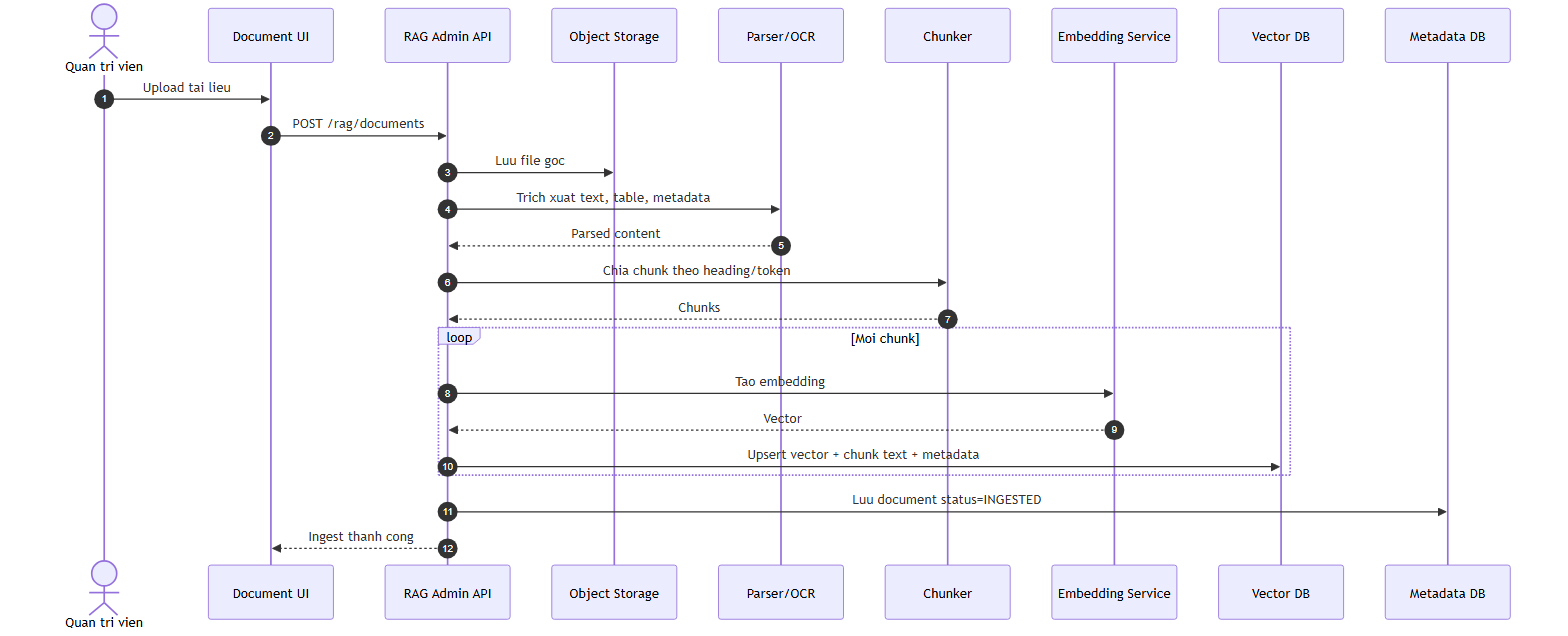
\includegraphics[width=\textwidth]{content/source/mermaid_sequence/seq_08.png}
    \caption{Luồng ingest tài liệu RAG}
\end{figure}

Theo sequence, quản trị viên tải tài liệu lên từ giao diện, backend nhận tệp, quét an toàn tên tệp, lưu tài liệu vào vùng nhập, sau đó khởi tạo pipeline xử lý nền. Trong pipeline này, tài liệu được chuyển sang văn bản sạch, phân đoạn, sinh embedding và cập nhật các kho lưu trữ cần thiết như vector store, document metadata hoặc graph. Sau khi ingest hoàn tất, tài liệu trở thành một phần của kho tri thức mà nhánh query có thể truy xuất.
